\chapter{Implementation}
\section{Differences between \ac{CPU} and \ac{GPGPU} hardware}
Before detailing the specific algorithms and configurations used by the RubiCL project, it is necessary to contrast two of the heterogeneous target architectures.

\ac{CPU} and \ac{GPGPU} architectures have diverged significantly due to differing traditional applications.

\ac{CPU} devices have had a long history of optimisation for sequential processing. As such, they have high clock-speeds and integrated hardware designed to increase instruction throughput; Modern processors rely heavily on \emph{branch predictors} and identifying opportunities for speedup via \emph{out-of-order execution}.

Conversely, the graphics pipeline tends to mainly utilise \ac{SIMD} operations. These consist of periods where the same few calculations are applied to vast quantities of data. With this execution pattern, complicated optimising hardware and higher clock-speeds are less favourable. Instead, hardware designers achieve incredible throughput by placing many massively parallel, yet simple, execution units on a single chipset.

In short, common \ac{GPGPU} hardware lacks many optimisations targeting single-threaded performance. More significantly, devices lack the ability to branch by jumping during execution. A flat sequence of instructions is processed by the hardware scheduler. Conditional logic is provided by condition-variable flags set on individual instructions. These masking flags state whether execution of each statement within a branch segment should occur.

The inability to jump causes code that branches to be necessarily inefficient. Any branching logic within a kernel will leave some execution units idling until the code path converges again.

Luckily, \ac{GPGPU} devices compensate by being exceptional at tasks resembling those that they were designed for: \ac{SIMD} computation patterns. A high-end \ac{GPU}, such as the \emph{Radeon R9 290X}, can contain as many as $44$ compute-units. Each compute unit is capable of scheduling $64$ concurrent \ac{SIMD} operations. At full utilisation, this vastly outperforms the raw instruction-rate of any \ac{CPU} device. The amount of parallelism possible in a latest-generation desktop \ac{GPGPU} is simply several orders of magnitude higher.

The goal of this project's implementation phase is to produce an easy-to-use library that presents significant throughput gains to an end-user performing common tasks.

\section{Parallel primitives}
\subsection{Map}
\verb|Map| is a higher-order function that mutates all elements in a provided input vector by applying a function parameter. It can be used to concisely describe a uniform alteration.
\verb|Map| is simple to parallelise since no sharing of each individual thread's state is required.
\paragraph*{Algorithm design}
\begin{algorithm}
  \caption{\emph{Map} higher-order function with sequential execution.}
  \label{alg:seqmap}

  \begin{algorithmic}
    \Function{SeqMap}{$f, A$}
      \ForAll{$a_i \in A$}
        \State{$a_i \Leftarrow$ \Call{$f$}{$a_i$}}
      \EndFor
    \EndFunction
  \end{algorithmic}
\end{algorithm}

Upon examining the sequential implementation of the \verb|map| primitive shown in Algorithm~\ref{alg:seqmap}, it is clear that iteration $i$ only reads and writes value $a_i$.

The dependency graph for a \verb|map| of $\|A\| = 6$ is shown in Figure~\ref{fig:mapgraph}.

\begin{figure}[h]
  \caption{\emph{Map} dependency graph}
  \label{fig:mapgraph}
  \begin{center}
    \begin{tikzpicture}
      [scale=.8,auto=left,every node/.style={circle}]

      \foreach \el/\x/\val in {n1/1/a_1, n2/2/a_2, n3/3/a_3, n4/4/a_4, n5/5/a_5, n6/6/a_6}
        \node (\el) at (2 * \x, 0) {$\val$};

      \foreach \el/\x/\val in {n1/1/a_1, n2/2/a_2, n3/3/a_3, n4/4/a_4, n5/5/a_5, n6/6/a_6}
        \path (\el) edge [anchor=center,loop above] node {} (\el);

    \end{tikzpicture}
  \end{center}
\end{figure}

When analysing data-dependency graphs, such as the one above, any partitioning that doesn't sever edges denotes a valid parallel strategy. Since Figure~\ref{fig:mapgraph} contains no inter-node dependencies, it is trivial to schedule the task concurrently on many compute units.

\algblockdefx[Pf]{PFor}{EndPFor}{\textbf{in parallel, for} }{\textbf{end parallel for}}
\begin{algorithm}
  \caption{\emph{Map} higher-order function with parallel execution.}
  \label{alg:parmap}

  \begin{algorithmic}
    \Function{ParMap}{$f, A$}
      \PFor{$a_i \in A$}
        \State{$a_i \Leftarrow$ \Call{$f$}{$a_i$}}
      \EndPFor
    \EndFunction
  \end{algorithmic}
\end{algorithm}

\paragraph*{Equivalent \ac{OpenCL} kernel design}
The \ac{OpenCL} execution model suggests performing tasks over a dataset by scheduling many distinct work-units. As a result, the side-effects of Algorithm~\ref{alg:parmap}'s loop body are now provided by the result of many individual kernel-function invocations. Algorithm~\ref{alg:oclmap} describes an \ac{OpenCL} kernel that performs \verb|map| computation with a size $\|A\|$ work-group.

\begin{algorithm}
  \caption{\emph{Map} higher-order function in OpenCL kernel form.}
  \label{alg:oclmap}

  \begin{algorithmic}
    \State{$f \Leftarrow$ \Call{MutationFunction}{}}

    \Function{MapKernel}{$A$}
      \State{\Call{DeclareVariables}{$f$}}
      \State{$i \Leftarrow$ \Call{GetGlobalID}{}}
      \State{$a_i \Leftarrow$ \Call{$f$}{$a_i$}}
    \EndFunction
  \end{algorithmic}
\end{algorithm}

\paragraph*{Alternative kernel investigation}
\subparagraph*{Motivation}
After producing a system that performs \verb|map| parallelisation akin to Algorithm~\ref{alg:oclmap}, suspicion arose over whether it was excessive to schedule one work-unit per element. With traditional threaded programming, there is a significant performance cost when creating each parallel subroutine. In addition, with many kernel invocations all writing to offsets in the globally-available $A$, it was theorised that large numbers of competing memory access requests would hamper throughput.

\subparagraph*{Kernel adaption}
In order to ensure that any anticipated scaling issues were avoided, a new kernel design was constructed. The alternate design avoids scheduling a number of work-units greater than the number of compute-units present.

\begin{algorithm}
  \caption{\emph{Map} higher-order function in reduced-work-unit OpenCL kernel form.}
  \label{alg:oclmap2}

  \begin{algorithmic}
    \State{$f \Leftarrow$ \Call{MutationFunction}{}}
    \State{$width \Leftarrow \ceil{\frac{\|A\|}{compute\_units}}$}


    \Function{MapKernel}{$A, width, \|A\|$}
      \State{\Call{DeclareVariables}{$f$}}
      \State{$i \Leftarrow$ \Call{GetGlobalID}{}}
      \State{$i_{initial} \Leftarrow i \times width$}
      \State{$i_{next} \Leftarrow (i + 1) \times width$}
      \For{$i \in ((i_{initial} \ldots (i_{next} - 1) \cap (i_{initial} \ldots (\|A\| - 1))$}
        \State{$a_i \Leftarrow$ \Call{$f$}{$a_i$}}
      \EndFor
    \EndFunction
  \end{algorithmic}
\end{algorithm}

The adapted kernel, now performing \verb|map| computation using a size $\|CU\|$ work-group, is presented in Algorithm~\ref{alg:oclmap2}.

\subparagraph*{Results}
After benchmarking the execution time of the kernels presented in Algorithms \ref{alg:oclmap} and \ref{alg:oclmap2}, no significant difference in performance was found. This suggests that the overhead for work-unit scheduling within the \ac{OpenCL} framework is very low. It also suggests that simultaneous access to neighbouring global-buffer elements does not affect latency worse than strided simultaneous access.

Influenced by these findings, the decision was made to use Algorithm~\ref{alg:oclmap} for \verb|map| tasks. This is due to the design being conceptually simpler, and therefore choosing the most basic solution that works well.
\todo{Verify this conclusion on desktop}

\subsection{Scan}
\verb|Reduce| is a higher-order function that takes an array and an initial `result' value (usually an identity value) and then repeatedly applies a combining function to produce an output.

The final result is equivalent to repeatedly updating the initial value with the output of itself and the next set member using the combiner. Using this technique, the input array is consumed once while the result is cumulatively generated. Any associative reduction function can be parallelised to increase throughput.

A well-known example of reduction is when the initial value is $0$ and the combining function is \verb|+(x, y)|. This results in \emph{summation} of an input dataset.

\verb|Scan| is similar to \verb|Reduce| in that it takes an input vector and a combining function.

Instead of returning the final result, Scan returns a vector that is equal to the intermediate values if the combining function was incrementally applied from one end of the dataset to the other. \verb|Scan| can also exploit a highly-parallel architecture when supplied with suitable operators.

\paragraph*{Algorithm design}
\begin{algorithm}
  \caption{\emph{Inclusive Scan} higher-order function with sequential execution.}
  \label{alg:seqscan}

  \begin{algorithmic}
    \Function{SeqScan}{$f, a_{-1}, A$}
      \ForAll{$a_i \in A$}
      \State{$a_i \Leftarrow$ \Call{$f$}{$a_{i-1} , a_i$}}
      \EndFor
    \EndFunction
  \end{algorithmic}
\end{algorithm}

Unlike sequential \verb|map|, iteration $i$ now reads from both $a_{i-1}$ and $a_{i}$ in addition to writing $a_i$. This produces a data-dependency graph with greater connectedness, shown in Figure~\ref{fig:scangraph}

\begin{figure}[h]
  \caption{\emph{Inclusive Scan} dependency graph}
  \label{fig:scangraph}
  \begin{center}
    \begin{tikzpicture}
      [scale=.8,auto=left,every node/.style={circle}]

      \node (init) at (0, 0) {$initial$};
      \foreach \el/\x/\val in {n1/1/a_1, n2/2/a_2, n3/3/a_3, n4/4/a_4, n5/5/a_5, n6/6/a_6}
        \node (\el) at (2 * \x, 0) {$\val$};


      \foreach \el/\prev in {n1/init, n2/n1, n3/n2, n4/n3, n5/n4, n6/n5} {
        \path (\el) edge [anchor=center,loop above] node {} (\el);
        \draw[->] (\el) -- (\prev);
      }

    \end{tikzpicture}
  \end{center}
\end{figure}

It is clear that no partitioning of this graph exists that does not sever edges. Therefore, this task is not embarrassingly parallel.

However, this does not mean that all hope is lost. It is possible to efficiently parallelise a \verb|scan| task, but it requires performing computation split over multiple \emph{stages}. One method for achieving this is demonstrated in Figure~\ref{fig:odd_even}.

\begin{figure}[h]
\begin{center}
  \includegraphics[width=0.8\textwidth]{./figures/oddeven.pdf}
  \caption{An example of parallelised \emph{inclusive scan} using the \emph{odd-even} algorithm, detailed in Algorithm~\ref{alg:parscan}}
  \label{fig:odd_even}
\end{center}
\end{figure}

\begin{algorithm}
  \caption{Odd-even style \emph{Scan} higher-order function with parallel execution.}
  \label{alg:parscan}

  \begin{algorithmic}
    \Function{ParScan}{$f, A$}
      \State{$level \Leftarrow 2$}

      \While{$level <= \|A\|$}
        \PFor{$l \in (level\ldots2 \times level\ldots\|A\|)$}
          \State{$A_l \Leftarrow$ \Call{$f$}{$A_l, A_{l - \frac{level}{2}}$}}
        \EndPFor
        \State{$level \Leftarrow 2 \times level$}
      \EndWhile

      \If{$level = \|A\|$}
      \State{$level \Leftarrow \frac{level}{2}$}
      \EndIf

      \While{$level > 1$}
      \PFor{$l \in (level + \frac{level}{2}\ldots2 \times level + \frac{level}{2}\ldots\|A\|)$}
          \State{$A_l \Leftarrow$ \Call{$f$}{$A_l, A_{l - \frac{level}{2}}$}}
        \EndPFor
        \State{$level \Leftarrow \frac{level}{2}$}
      \EndWhile

    \EndFunction
  \end{algorithmic}
\end{algorithm}

A parallel algorithm's \emph{cost} is defined as its asymptotic runtime multiplied by the required number of compute-units.


The \emph{odd-even} prefix sum algorithm can process a dataset of size $n$ in $O(\log n) + \frac{O(n)}{\|CU\|}$ stages of execution. This gives a cost of $O(\|CU\| \log n) + O(n)$.
Importantly, it is \emph{cost-optimal}, meaning that its cost is equal to that of the best-known sequential algorithm, when $\|CU\| = O(\frac{n}{\log n})$. This is an entirely reasonable assumption given large datasets and the number of compute-units ($4-48$) present on commodity \ac{OpenCL} devices.

This discovery suggests that it is possible to increase the throughput of \verb|scan| tasks significantly, by scheduling them across massively parallel \ac{OpenCL} devices.

\subsection{Scatter}
The \verb|Scatter| primitives receives an input array $A$, an array of indices $I$, and an output array $B$. It updates $B$ such that $B_{I_i} \Leftarrow A_i$. Put otherwise, it inserts the value given at offset $i$ of $A$ into $B$, at the position given by the value at offset $i$ of $I$.

\verb|Scatter| is useful for reordering a collection or projecting a subset of an input dataset into an output dataset.

\begin{algorithm}
  \caption{\emph{Scatter} primitive with sequential execution.}
  \label{alg:seqscatter}

  \begin{algorithmic}
    \Function{SeqScatter}{$A, I, B$}
      \ForAll{$a_i \in A$}
      \State{$B_{I_i} \Leftarrow A_i$}
      \EndFor
    \EndFunction
  \end{algorithmic}
\end{algorithm}

\paragraph*{Two types of scatter}
It is important to draw attention to an important distinction in types of \verb|scatter| operation. \emph{Permutation Scatter} is defined as a scatter operation where all $i \in I$ are unique. Therefore, there are no two writes to the same destination in $B$. Other forms of \verb|scatter| increase complexity, as rules that state how to handle write collisions within the transaction must be introduced.

Luckily, for this project's needs we only need to analyse the simpler \emph{permutation scatter}. We can assume that no two writes to the same destination offset will occur.

\begin{figure}[h]
  \caption{\emph{Permutation Scatter} dependency graph}
  \label{fig:scatgraph1}
  \begin{center}
    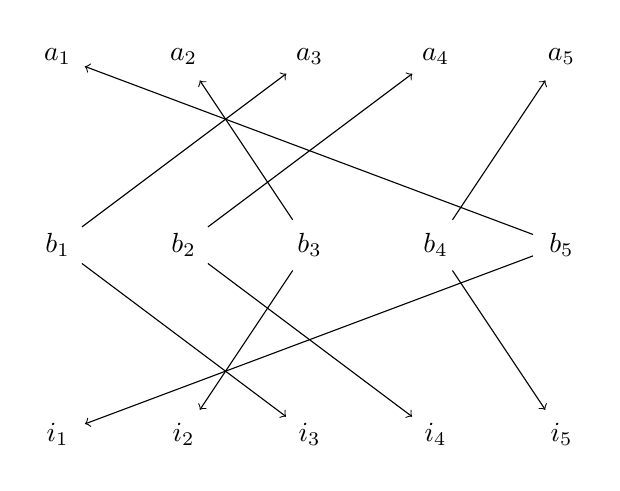
\begin{tikzpicture}
      [scale=.8,auto=left,every node/.style={circle}]

      \foreach \x in {1, 2, 3, 4, 5} {
        \node (a\x) at (2 * \x, 3) {$a_{\x}$};
        \node (b\x) at (2 * \x, 0) {$b_{\x}$};
        \node (i\x) at (2 * \x, -3){$i_{\x}$};
      }

      \foreach \s/\d in {1/5, 2/3, 3/1, 4/2, 5/4}{
        \draw[->] (b\d) -- (a\s);
        \draw[->] (b\d) -- (i\s);
      }

    \end{tikzpicture}
  \end{center}
\end{figure}
A data-dependency graph for a typical scatter operation is shown in Figure~\ref{fig:scatgraph1}.
At first, it may appear complicated. However, when nodes $b_i \in B$ are reordered by their data-source, a valid partitioning becomes clear. The result of this simplification is shown in Figure~\ref{fig:scatgraph2}.

\begin{figure}[h]
  \caption{\emph{Permutation Scatter} dependency graph, simplified.}
  \label{fig:scatgraph2}
  \begin{center}
    \begin{tikzpicture}
      [scale=.8,auto=left,every node/.style={circle}]

      \foreach \s/\d in {1/5, 2/3, 3/1, 4/2, 5/4}{
        \node (a\s) at (2 * \s, 2) {$a_{\s}$};
        \node (b\d) at (2 * \s, 0) {$b_{\d}$};
        \node (i\s) at (2 * \s, -2){$i_{\s}$};
        \draw[->] (b\d) -- (a\s);
        \draw[->] (b\d) -- (i\s);
      }
    \end{tikzpicture}
  \end{center}
\end{figure}

This suggests that \verb|scatter|, when using unique indices, is \emph{embarassingly parallel}. Like \verb|map|, this produces an easy-to-understand parallel conversion, shown in Algorithm~\ref{alg:parscatter}.

\begin{algorithm}
  \caption{\emph{Permutation Scatter} primitive with parallel execution.}
  \label{alg:parscatter}

  \begin{algorithmic}
    \Function{ParScatter}{$A, I, B$}
      \PFor{$a_i \in A$}
      \State{$B_{I_i} \Leftarrow A_i$}
      \EndPFor
    \EndFunction
  \end{algorithmic}
\end{algorithm}
\subsection{Filter}

\todo{Explain how this just uses the previous operators}

\subsection{Sort}


\section{Subcomponents}

\section{Functionality Testing}

\section{Performance Testing}
